\documentclass[aspectratio=169]{beamer}

\usepackage[utf8]{inputenc} % codificacao de caracteres
\usepackage[T1]{fontenc}    % codificacao de fontes
\usepackage[brazil]{babel}  % idioma


\usetheme{Berlin}         % tema
\usecolortheme{seahorse}      % cores

\usefonttheme[onlymath]{serif} % fonte modo matematico
\usepackage{amsthm}

% Titulo
\title[\sc{Processamento de imagens}]{Processamento de imagens - Morfologia Matemática}
\author[Alano Martins Pinto]{Alano Martins Pinto e Gildácio Sá}
\institute{UECE - Universidade Estadual do Ceará} % opcional
\date{\today}


% Colocando numero de paginas no slide
\setbeamertemplate{footline}[frame number]

% Desativando os botoes de navegacao
\beamertemplatenavigationsymbolsempty

% Tela cheia\section{section1}

\hypersetup{pdfpagemode=FullScreen}

% Layout da pagina
\hypersetup{pdfpagelayout=SinglePage}

% Definicao de novos comandos
\providecommand{\sin}{} \renewcommand{\sin}{\hspace{2pt}\textrm{sen}}
\providecommand{\tan}{} \renewcommand{\tan}{\hspace{2pt}\textrm{tg}}
\newcommand{\R}{\mathbb{R}}

% Capa - requer o TikZ
\newcommand{\capa}{
    \begin{tikzpicture}[remember picture,overlay]
        \node at (current page.south west)
            {\begin{tikzpicture}[remember picture, overlay]
                \fill[shading=radial,top color=orange,bottom color=orange,middle color=red] (0,0) rectangle (\paperwidth,\paperheight);
            \end{tikzpicture}
          };
    \end{tikzpicture}
}


% Definicao de novos ambientes
\theoremstyle{Definition}
\newtheorem{defn}{Defini\c c\~ao}
\newtheorem{teo}[theorem]{Teorema}
\newtheorem{ex}[theorem]{Exemplo}
\newtheorem{eq}[theorem]{Equa\c c\~ao}


\usepackage{etoolbox}
\newcommand{\zerodisplayskips}{%
  \setlength{\abovedisplayskip}{0pt}%
  \setlength{\belowdisplayskip}{0pt}%
  \setlength{\abovedisplayshortskip}{0pt}%
  \setlength{\belowdisplayshortskip}{0pt}}
\appto{\normalsize}{\zerodisplayskips}
\appto{\small}{\zerodisplayskips}
\appto{\footnotesize}{\zerodisplayskips}



\begin{document}

\begin{frame}
	\titlepage
\end{frame}


\begin{frame}
	\frametitle{Tópicos}
	\begin{itemize}
		\item Conceitos
		\item Teoria dos conjuntos
		\item Operações lógicas
		\item Dilatação e Erosão
		\item Abertura e fechamento
		\item Transformação Hit-or-miss
		\item Extração de bordas
		\item Extração de componentes conexas
		\item Conver Hull
		\item Thinning
		\item Thickening
		\item Esqueleto
		\item Poda
		\item Morfologia em escala de cinza
	\end{itemize}

\end{frame}


% Frame 4: teoria dos conjuntos
\begin{frame}\frametitle{Teoria dos conjuntos}

União: $C = A \cap B $ 

Interceção: $C = A \cup B $ 

Subtração: $C = A - B $ 

Complementar: $A^{c} = \{w \,|\, w \not\in A  \}$ 

  \begin{figure}[h]
    \centering
    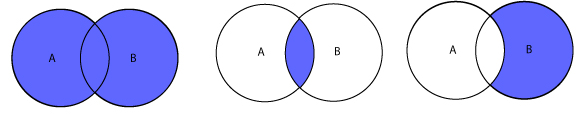
\includegraphics[height=0.3\paperheight]{imagens/basic_sets}
    %\includegraphics[height=6cm]{figCoordEsf02}
    \caption{Propriedades básicas de conjuntos}\label{figConjuntos}
  \end{figure}

\end{frame}


% Frame 4: expressoes matematicas
\begin{frame}
	\frametitle{Complementar}
	
	\begin{defn}
    	Conjunto de pontos que não estão em A
	\end{defn}

	\begin{eq}
    	$A^{c} = \{w \,|\, w \not\in A  \}$ 
	\end{eq}
	
  \begin{figure}[h]
    \centering
    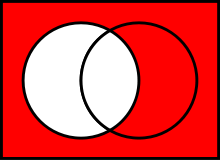
\includegraphics[height=0.3\paperheight]{imagens/complementar}
    %\includegraphics[height=6cm]{figCoordEsf02}
    \caption{Complementar de conjuntos}\label{figComplementar}
  \end{figure}
\end{frame}

\begin{frame}
	\frametitle{Translação}
	
	\begin{defn}
    	Move a origem de A para o ponto z
	\end{defn}

	\begin{eq}
    	$(A)z = \{c \,|\, c = a + z$, para $ a \in A  \}$ 
	\end{eq}
	
  \begin{figure}[h]
    \centering
    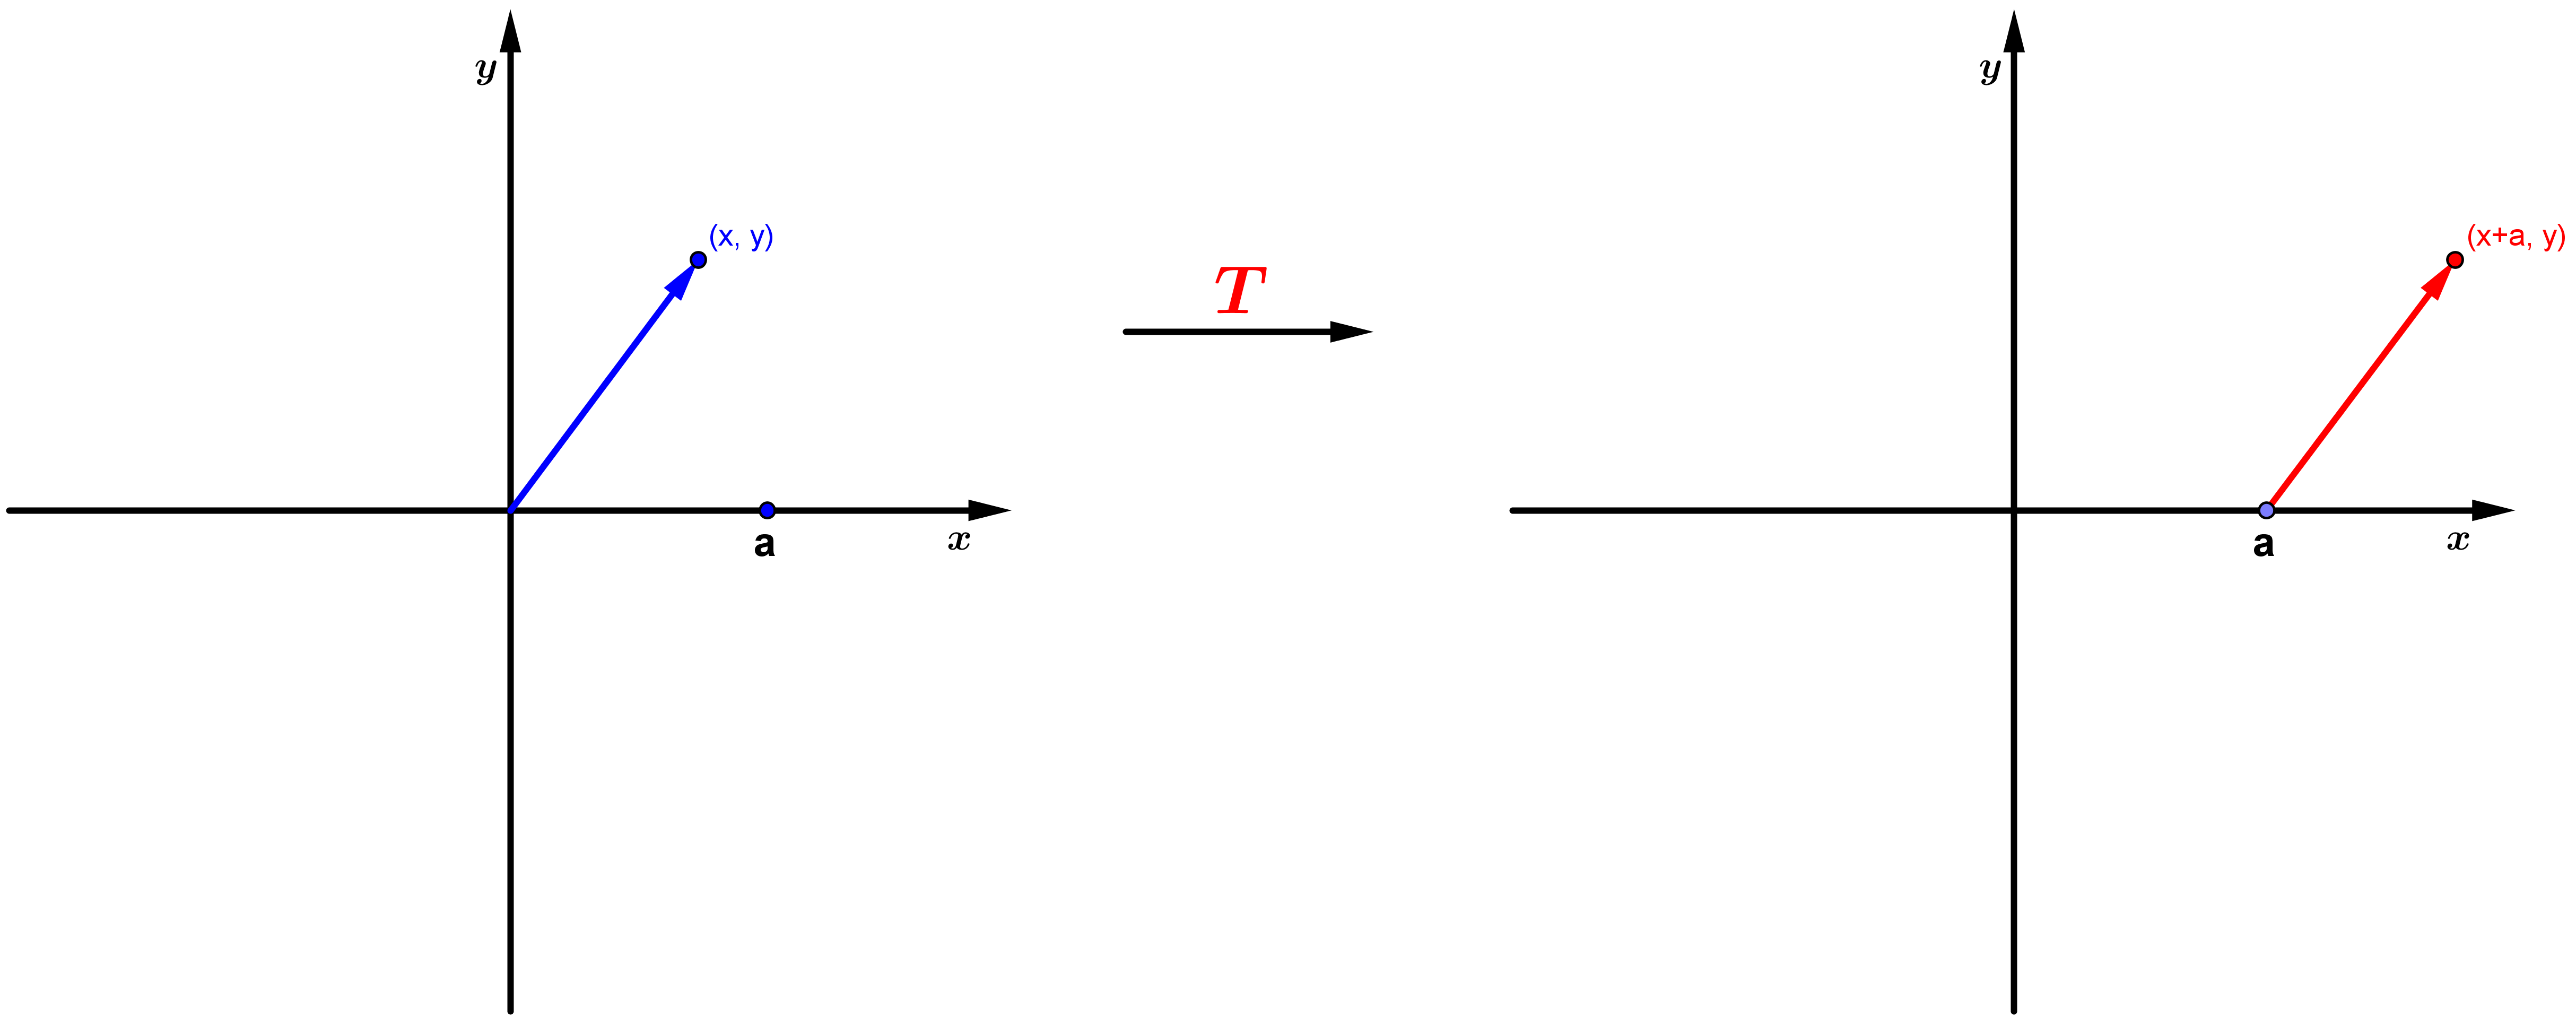
\includegraphics[height=0.3\paperheight]{imagens/translacao}
    %\includegraphics[height=6cm]{figCoordEsf02}
    \caption{Translação em vetor}\label{figTranslacao}
  \end{figure}
\end{frame}

\begin{frame}
	\frametitle{Reflexão}
	
	\begin{defn}
    	Reflete todos os elementos de B sobrem a origme desse conjunto
	\end{defn}

	\begin{eq}
    	$ B = \{w \,|\, w = -b$, para $ b \in B  \}$ 
	\end{eq}
	
  \begin{figure}[h]
    \centering
    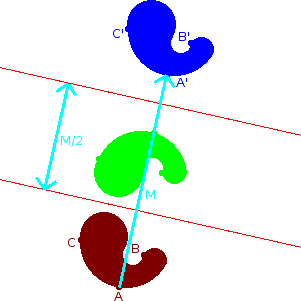
\includegraphics[height=0.3\paperheight]{imagens/reflect}
    %\includegraphics[height=6cm]{figCoordEsf02}
    \caption{Reflexão em figura}\label{figReflexao}
  \end{figure}
\end{frame}

\begin{frame}
	\frametitle{Operações lógicas (Binário) }
	
	\begin{columns}
		\begin{column}{0.3\textwidth}
		   \begin{itemize}
				\item NOT
				\item AND
				\item OR
				\item XOR
				\item NOT-AND
			\end{itemize}
		\end{column}
		\begin{column}{0.7\textwidth}  %%<--- here
    		\begin{figure}[h]
	   	 		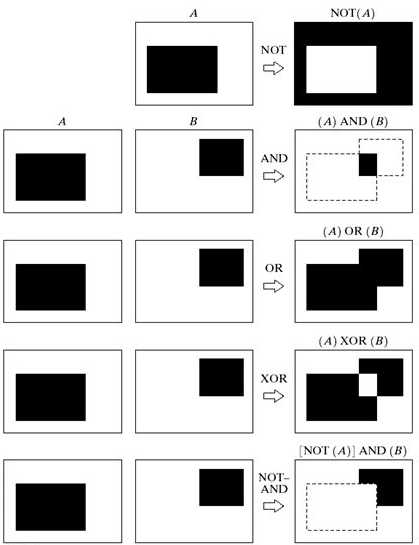
\includegraphics[width=4.4cm]{imagens/logical}
			    \caption{Operações lógicas}\label{figLogical}
	  		\end{figure}
		\end{column}
	\end{columns}
\end{frame}

\begin{frame}
	\frametitle{Extração de bordas}
	
	\begin{defn}
    	Extrai bordas do pixels frontal. Realiza uma erosão e após a diferença do conjunto A com o resultado.
	\end{defn}
	
	\begin{eq}
    	$ \beta(A) = A  - (A \circleddash B)$ 
	\end{eq}
	
	\begin{columns}
		\begin{column}{0.5\textwidth}
			\begin{figure}[h]
	  		 	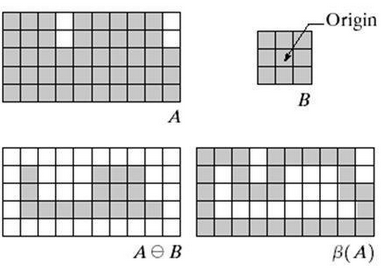
\includegraphics[width=4cm, height=0.25\paperheight]{imagens/border_ex1}
				\caption{Extração de bordas 1}\label{figLogical}
			\end{figure}
		\end{column}
		\begin{column}{0.5\textwidth}
			\begin{figure}[h]
			   	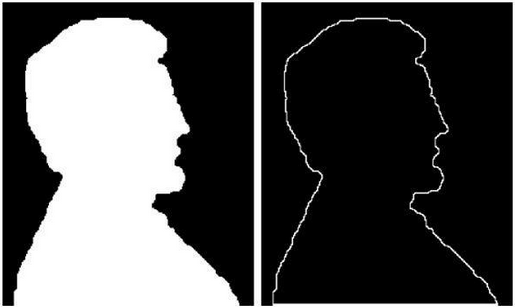
\includegraphics[width=4cm, height=0.25\paperheight]{imagens/border_ex2}
				\caption{Extração de bordas 2}\label{figLogical}
			\end{figure}
		\end{column}
	\end{columns}
	
\end{frame}

\begin{frame}
	\frametitle{Preenchimento de regiões}
	
	\begin{defn}
    	Preenche ua região em A, dado um ponto inicial p.
	\end{defn}
	
	\begin{eq}
    	$ X_k = ( X_{k-1} \bigoplus B) \cap A^c \qquad k = 1, 2, 3$   
	\end{eq}
	
	\begin{columns}
		\begin{column}{0.5\textwidth}
			\begin{figure}[h]
	  		 	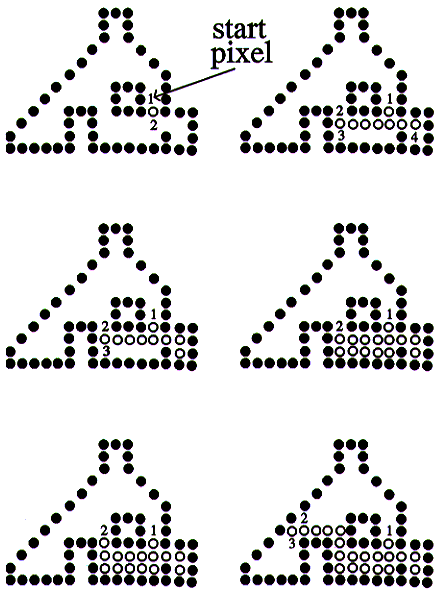
\includegraphics[height=0.3\paperheight]{imagens/fill}
				\caption{Preenchimento de regions}\label{figLogical}
			\end{figure}
		\end{column}
		\begin{column}{0.5\textwidth}
			\begin{figure}[h]
			   	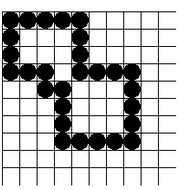
\includegraphics[width=4cm, height=0.3\paperheight]{imagens/fill2}
				\caption{Preenchimento de regions}\label{figLogical}
			\end{figure}
		\end{column}
	\end{columns}
	
\end{frame}

\begin{frame}
	\frametitle{Extração de componentes conexos}
	
	\begin{defn}
    	Encontra um componente conectado X em A.
	\end{defn}
	
	\begin{eq}
    	$ X_k = ( X_{k-1} \bigoplus B) \cap A \qquad k = 1, 2, 3$   
	\end{eq}
	
	\begin{columns}
		\begin{column}{0.5\textwidth}
			\begin{figure}[h]
	  		 	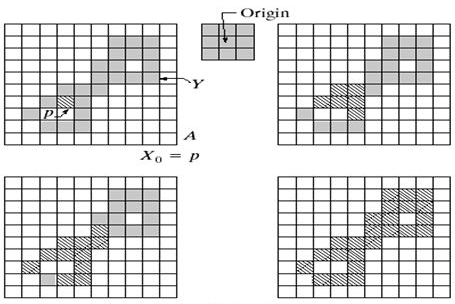
\includegraphics[height=0.3\paperheight]{imagens/conecteds}
				\caption{Componentes conectos}\label{figLogical}
			\end{figure}
		\end{column}
		\begin{column}{0.5\textwidth}
			\begin{figure}[h]
			   	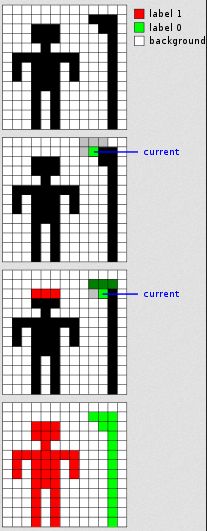
\includegraphics[width=4cm, height=0.3\paperheight]{imagens/conecteds2}
				\caption{Componentes conectos}\label{figLogical}
			\end{figure}
		\end{column}
	\end{columns}
	
\end{frame}

\begin{frame}
	\frametitle{Convex hull}
	
	\begin{defn}
		Encontra o envelopamento convexo de um conjunto A
	\end{defn}
	
	\begin{eq}
	
		\begin{align*}
			X^i_k& = ( X_{k-1} \circledast B^i) \cup A \qquad i = 1, 2, 3, 4 \qquad k = 1, 2, 3,..
		\end{align*}

	\end{eq}
	
	\begin{columns}
		\begin{column}{0.5\textwidth}
			\begin{figure}[h]
	  		 	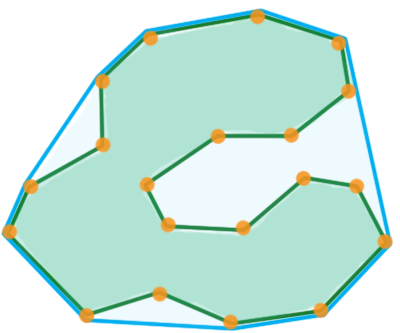
\includegraphics[height=0.15\paperheight]{imagens/convex_hull}
				\caption{Preenchimento de regions}\label{figLogical}
			\end{figure}
		\end{column}
		\begin{column}{0.5\textwidth}
			\begin{figure}[h]
			   	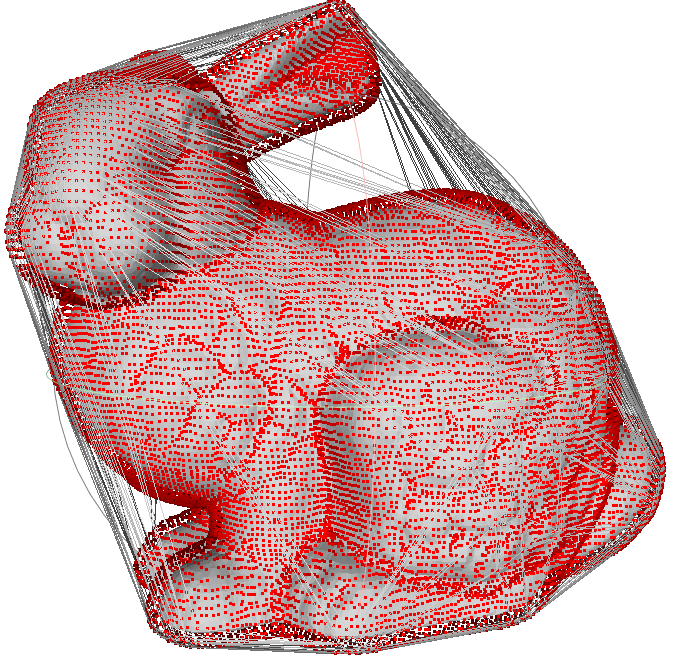
\includegraphics[height=0.15\paperheight]{imagens/convex_hull2}
				\caption{Preenchimento de regions}\label{figLogical}
			\end{figure}
		\end{column}
	\end{columns}
	
\end{frame}


\begin{frame}
	\frametitle{Afinamento}
	
	\begin{defn}
		Encontra o envelopamento convexo de um conjunto A
	\end{defn}
	
	\begin{eq}
	$ A \otimes B = A - (A \circledast B)$  OU\\
	$ A\cap (A \circledast B)^c$

	\end{eq}
	
	
\end{frame}

\begin{frame}
	\frametitle{Afinamento}
	
	\begin{figure}[h]
	 	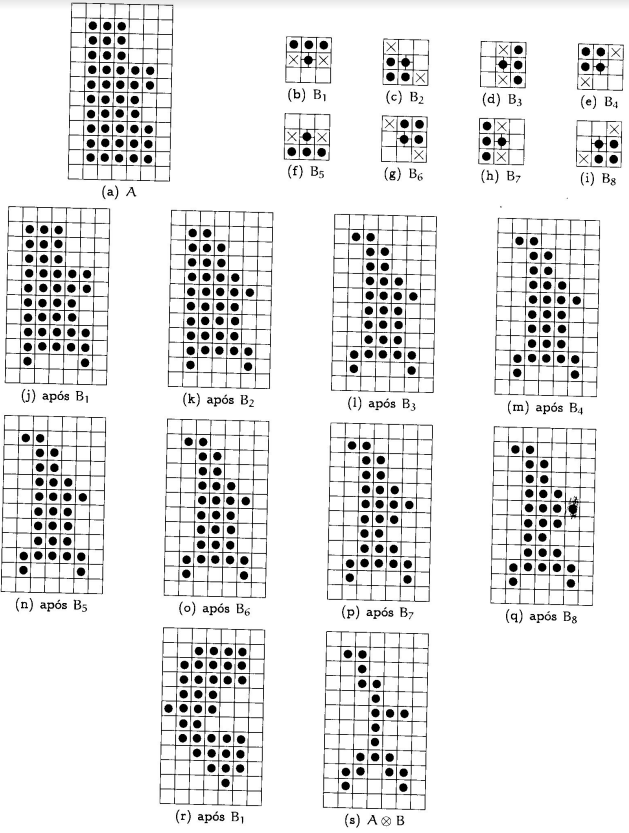
\includegraphics[width=0.6\paperwidth,height=0.6\paperheight]{imagens/afinamento}
		\caption{Afinamento}\label{figLogical}
	\end{figure}
	
\end{frame}

\begin{frame}
	\frametitle{Espessamento}
	
	\begin{defn}
		Aumenta a espessura de um conjunto A
	\end{defn}
	
	\begin{eq}
			$ A \odot B = A \cup (A \circledast B) $
	\end{eq}
	
\end{frame}

\begin{frame}
	\frametitle{Espessamento}
	
	\begin{figure}[h]
	 	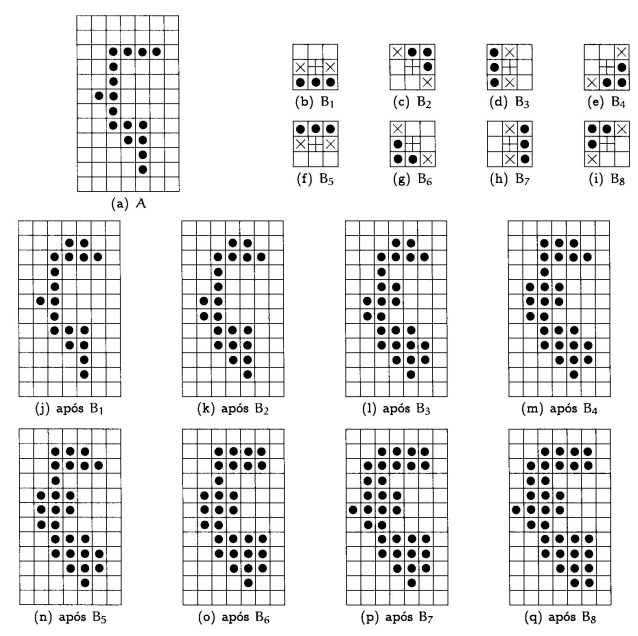
\includegraphics[width=0.6\paperwidth,height=0.6\paperheight]{imagens/espessamento}
		\caption{Espessamento}\label{figLogical}
	\end{figure}
	
\end{frame}

\begin{frame}
	\frametitle{Esqueleto}
	
	\begin{defn}
		Processo de redução da região foreground, preservando a extensão e conectividade.
	\end{defn}
	
	\begin{eq}
		\begin{align*}
				S(A) = \bigcup^k_{k=0} \{ (A \circleddash kB) - [(A \circleddash kB) \circ B] \}
		\end{align*}
	\end{eq}
	
	Reconstrução de A:
	
	\begin{eq}
		\begin{align}
				S(A) = \bigcup^k_{k=0} \{ (A \circleddash kB) - [(A \circleddash kB) \circ B] \}
		\end{align}
	\end{eq}
		
\end{frame}

\begin{frame}
	\frametitle{Esqueleto}
	
	\begin{figure}[h]
	 	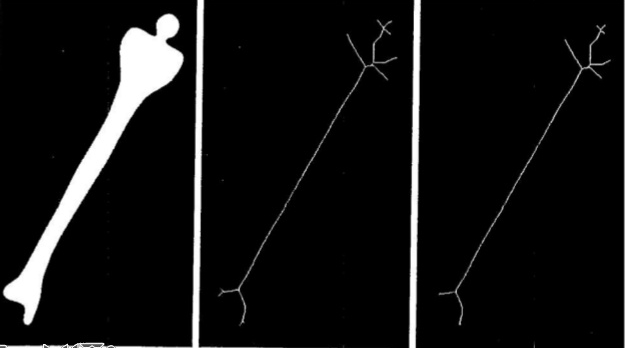
\includegraphics[width=0.6\paperwidth,height=0.6\paperheight]{imagens/skeleton1}
		\caption{Esqueleto}\label{figLogical}
	\end{figure}
	
\end{frame}

\begin{frame}
	\frametitle{Poda}
	
	\begin{defn}
		Aumenta a espessura de um conjunto A
	\end{defn}
	
	\begin{eq}
			\begin{align}
				X_1 &= A \otimes B \\
				X_2 &= \bigcup^8_{k=1} (X_1 \circledast B^k) \\
				X_3 &= (X_2 \oplus H) \cap A \\
				X_4 &= X_1 \cup X_3
		\end{align}
	\end{eq}
	
\end{frame}

\begin{frame}
	\frametitle{Poda}
	
	\begin{figure}[h]
	 	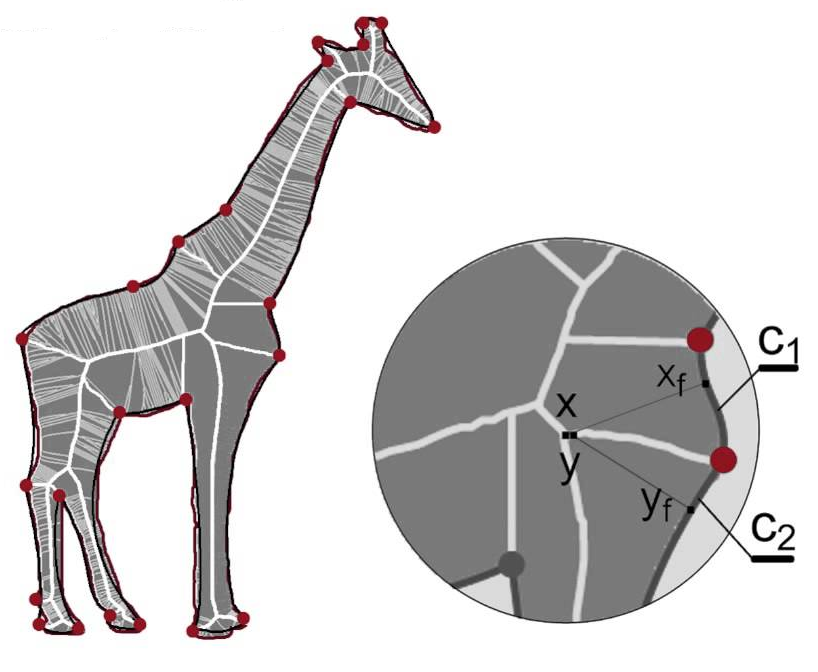
\includegraphics[width=0.6\paperwidth,height=0.6\paperheight]{imagens/prunning}
		\caption{Poda}\label{figLogical}
	\end{figure}
	
\end{frame}

\begin{frame}
	\frametitle{Morfologia - Imagens monocromáticas}
	
	\ \begin{itemize}
		\item NOT
		\item AND
		\item OR
		\item XOR
		\item NOT-AND
	\end{itemize}
	
	\begin{eq}
	$ A \otimes B = A - (A \circledast B)$  OU\\
	$ A\cap (A \circledast B)^c$

	\end{eq}
	
	
\end{frame}

\end{document}